\section{Experimentación Y Resultados}

\subsection{Casos de prueba}
   A continuación se listarán los casos utilizados y después se compararán los resultados.

	\begin{itemize}
		\item MOVIES: Este caso incluye 5797 páginas
		\item ABORTION: Este caso incluye 2293 páginas
		\item GENETIC: Este caso incluye 3468 páginas
		\item STANFORD: Este caso incluye 281903 páginas
		\item GOOGLE: Este caso incluye 916428 páginas
	\end{itemize}   

\subsection{Comparación de Normas}

En esta sección vamos a mostrar como evoluciona la norma Manhattan (también conocida como distancia L1) entre dos vectores a medida que se suceden las iteraciones.
La norma Manhattan es la distancia entre dos vectores, o en otras palabras, la suma de la diferencia coordenada a coordenada en modulo:

\begin{figure}[h!]
   \centering
    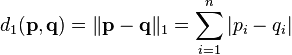
\includegraphics[width=0.5\textwidth]{imagenes/norma_manhattan.png}
\end{figure}


\subsubsection {PageRank}

Para evaluar el comportamiento de la norma manhattan variando la probabilidad del navegante aleatorio, el cual de ahora en más lo denotaremos como el parámetro \textbf{c}

Los casos de prueba se corrieron sin un limite entre normas pero si con un limite de 1000 iteraciones, ya que, según lo que investigamos, con un c 	$\approx$ 0.15 la matriz suele converger en un máximo de 50 iteraciones, que por lo que se puede observar suele ser proporcional esta relación a medida que aumenta el c.

A continuación se muestran los resultados para cuatro tests de como evoluciona la norma a lo largo de las iteraciones y como varía la misma con distintos c, y que luego discutiremos más adelante:

\begin{figure}
\begin{center}
       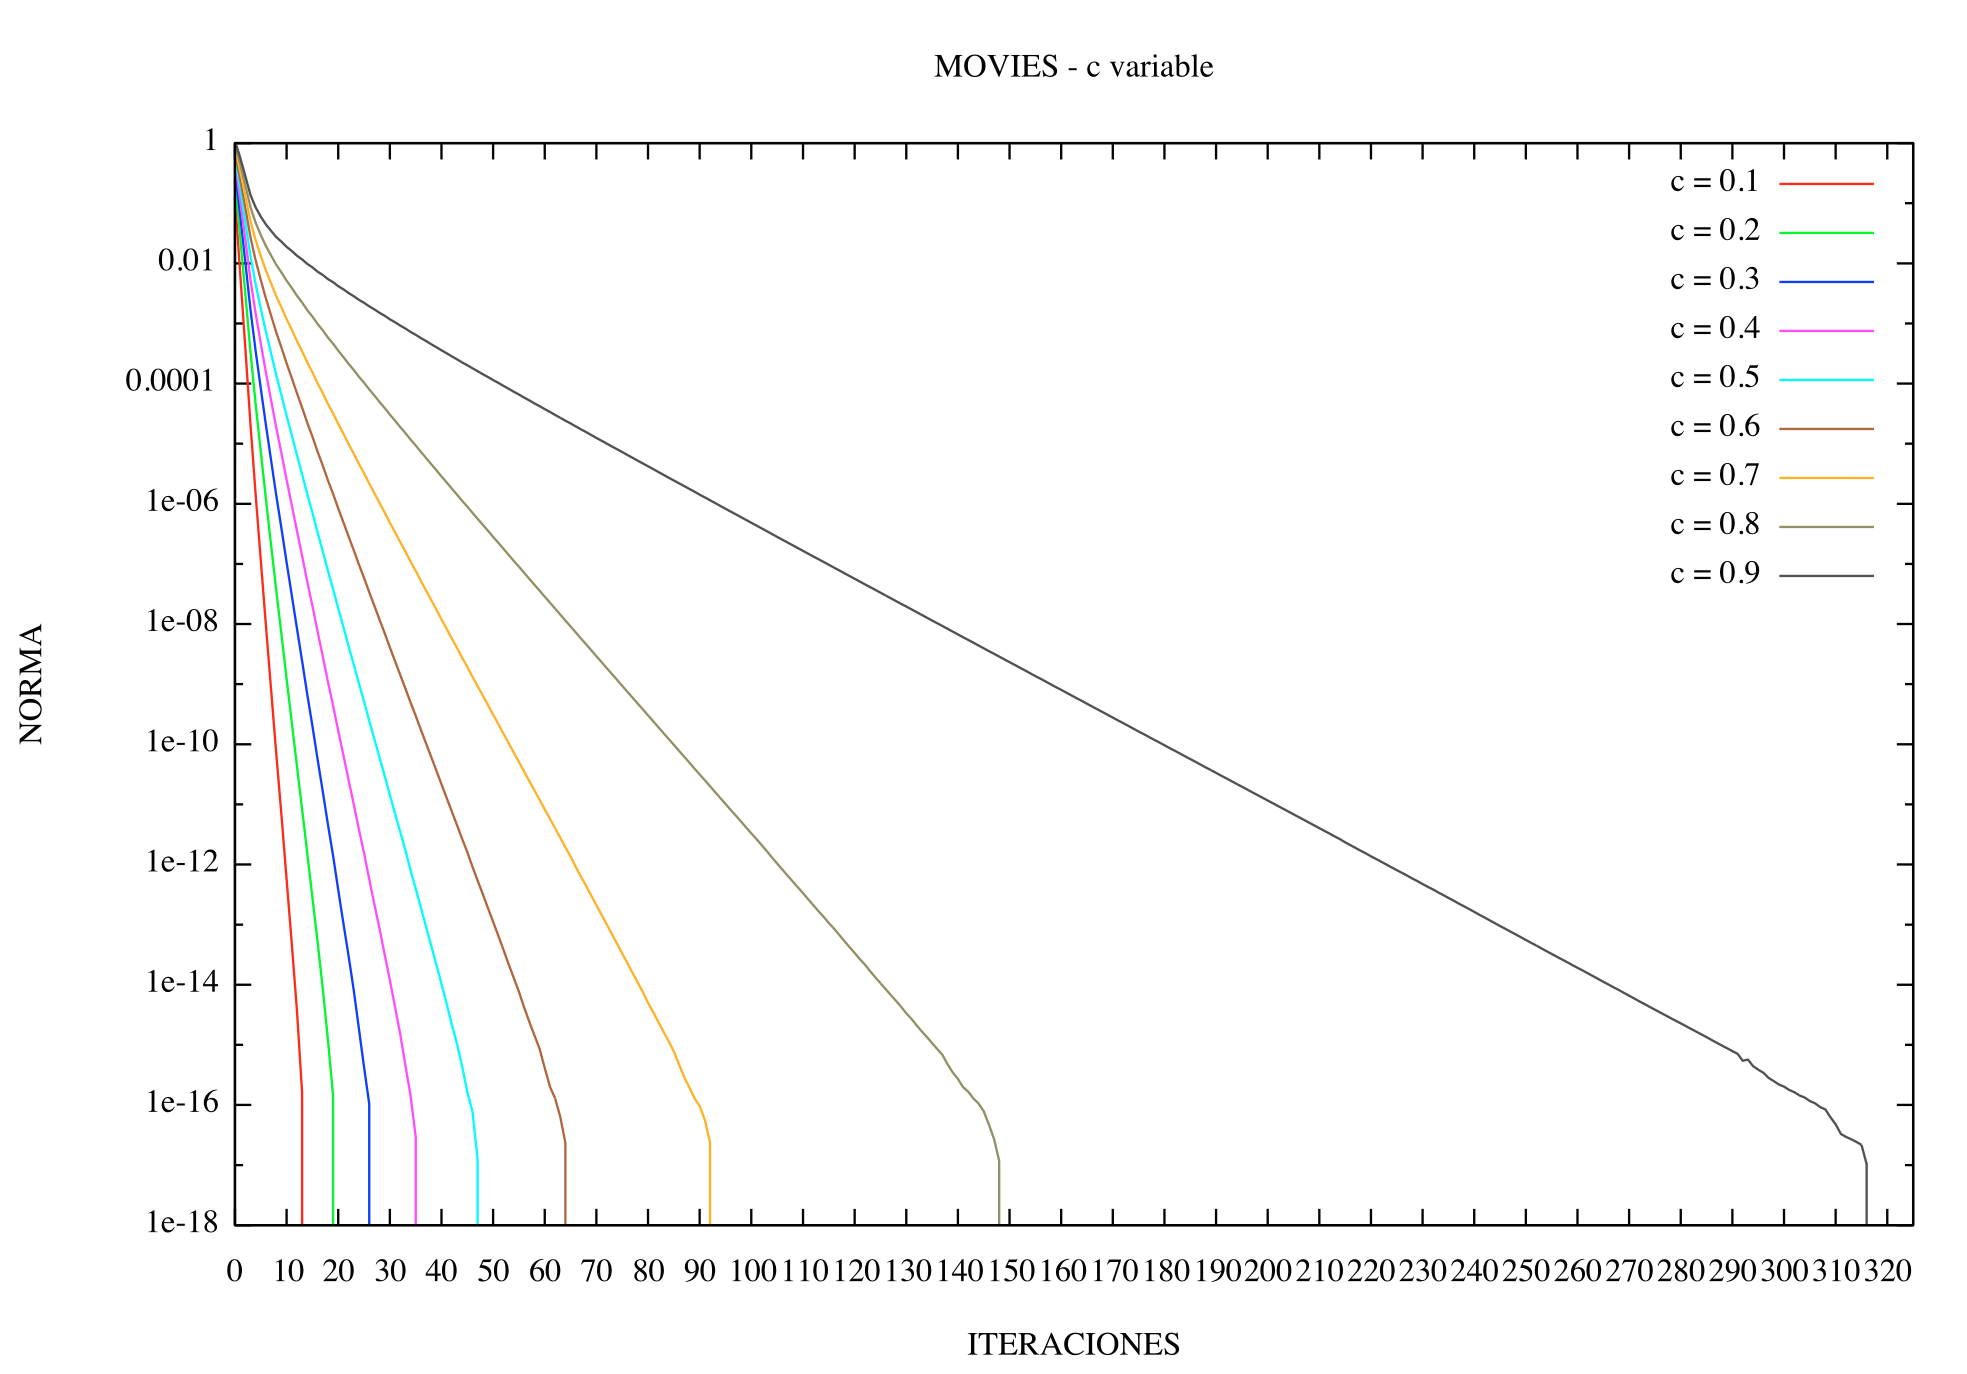
\includegraphics[scale=0.5]{imagenes/pagerank_movies_norma.png}
        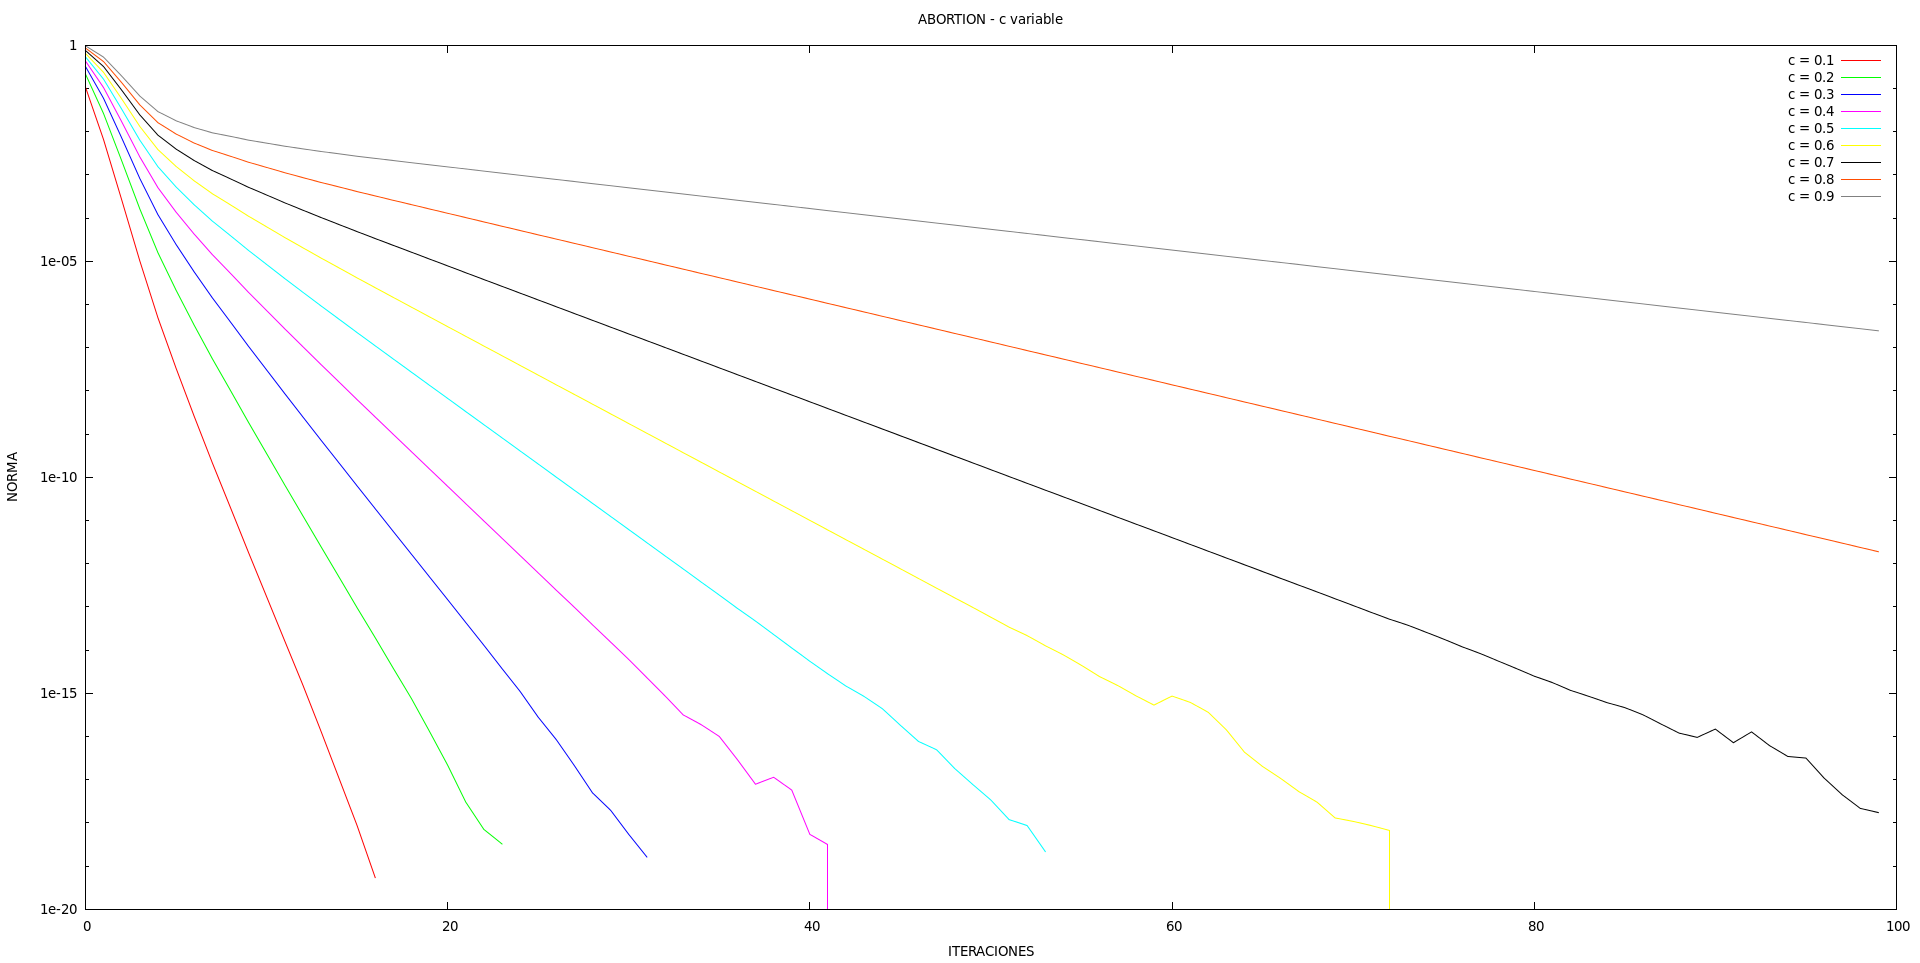
\includegraphics[scale=0.5]{imagenes/pagerank_abortion_norma.png}
       \end{center}
\end{figure}

\begin{figure}
\begin{center}
    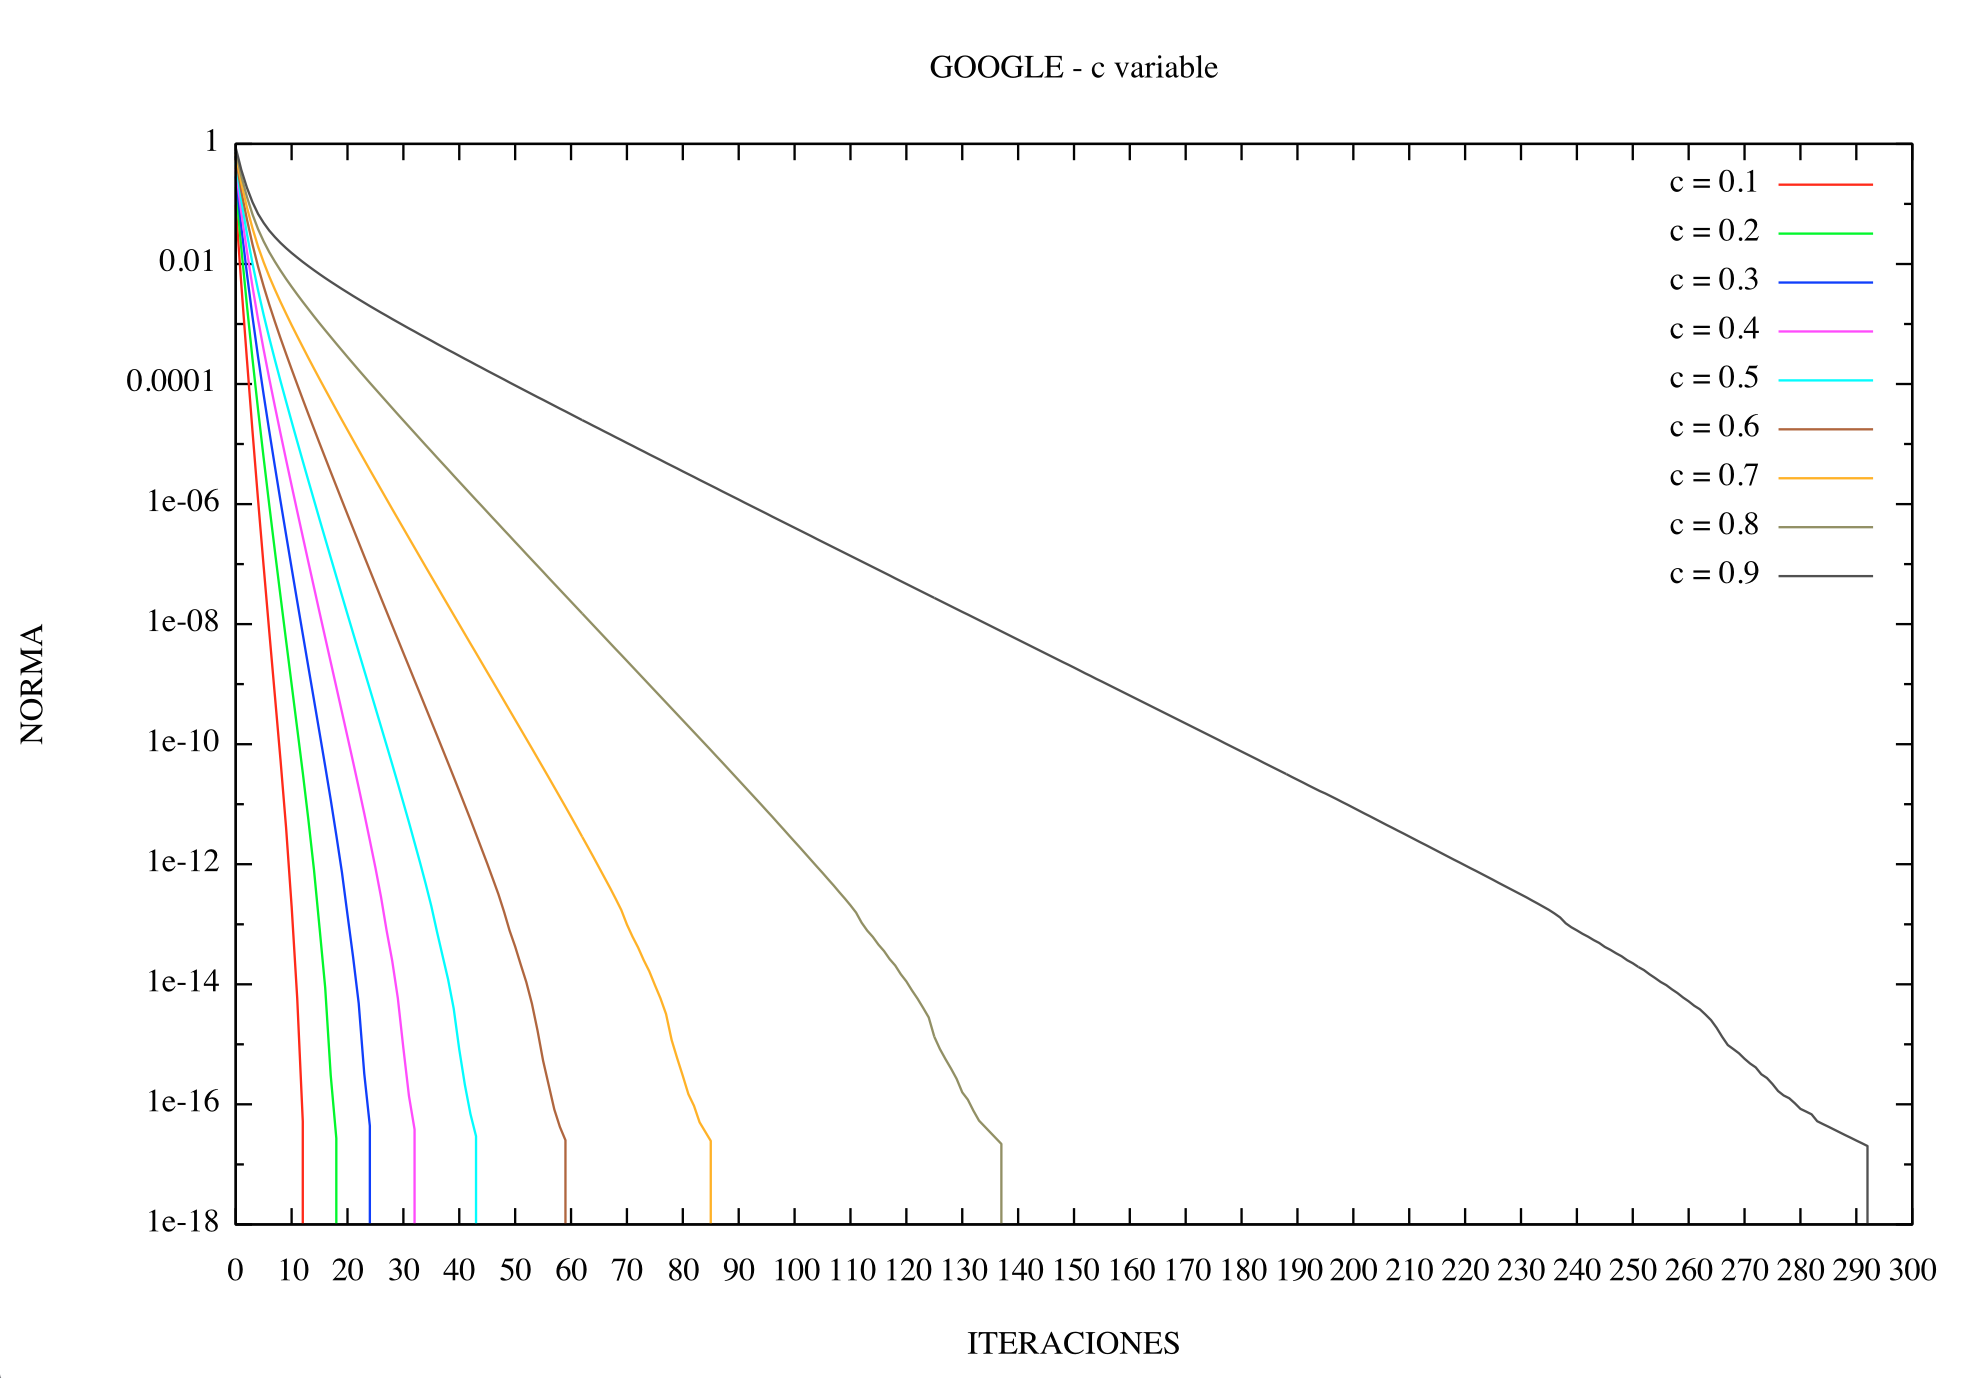
\includegraphics[scale=0.5]{imagenes/pagerank_google_norma.png}
  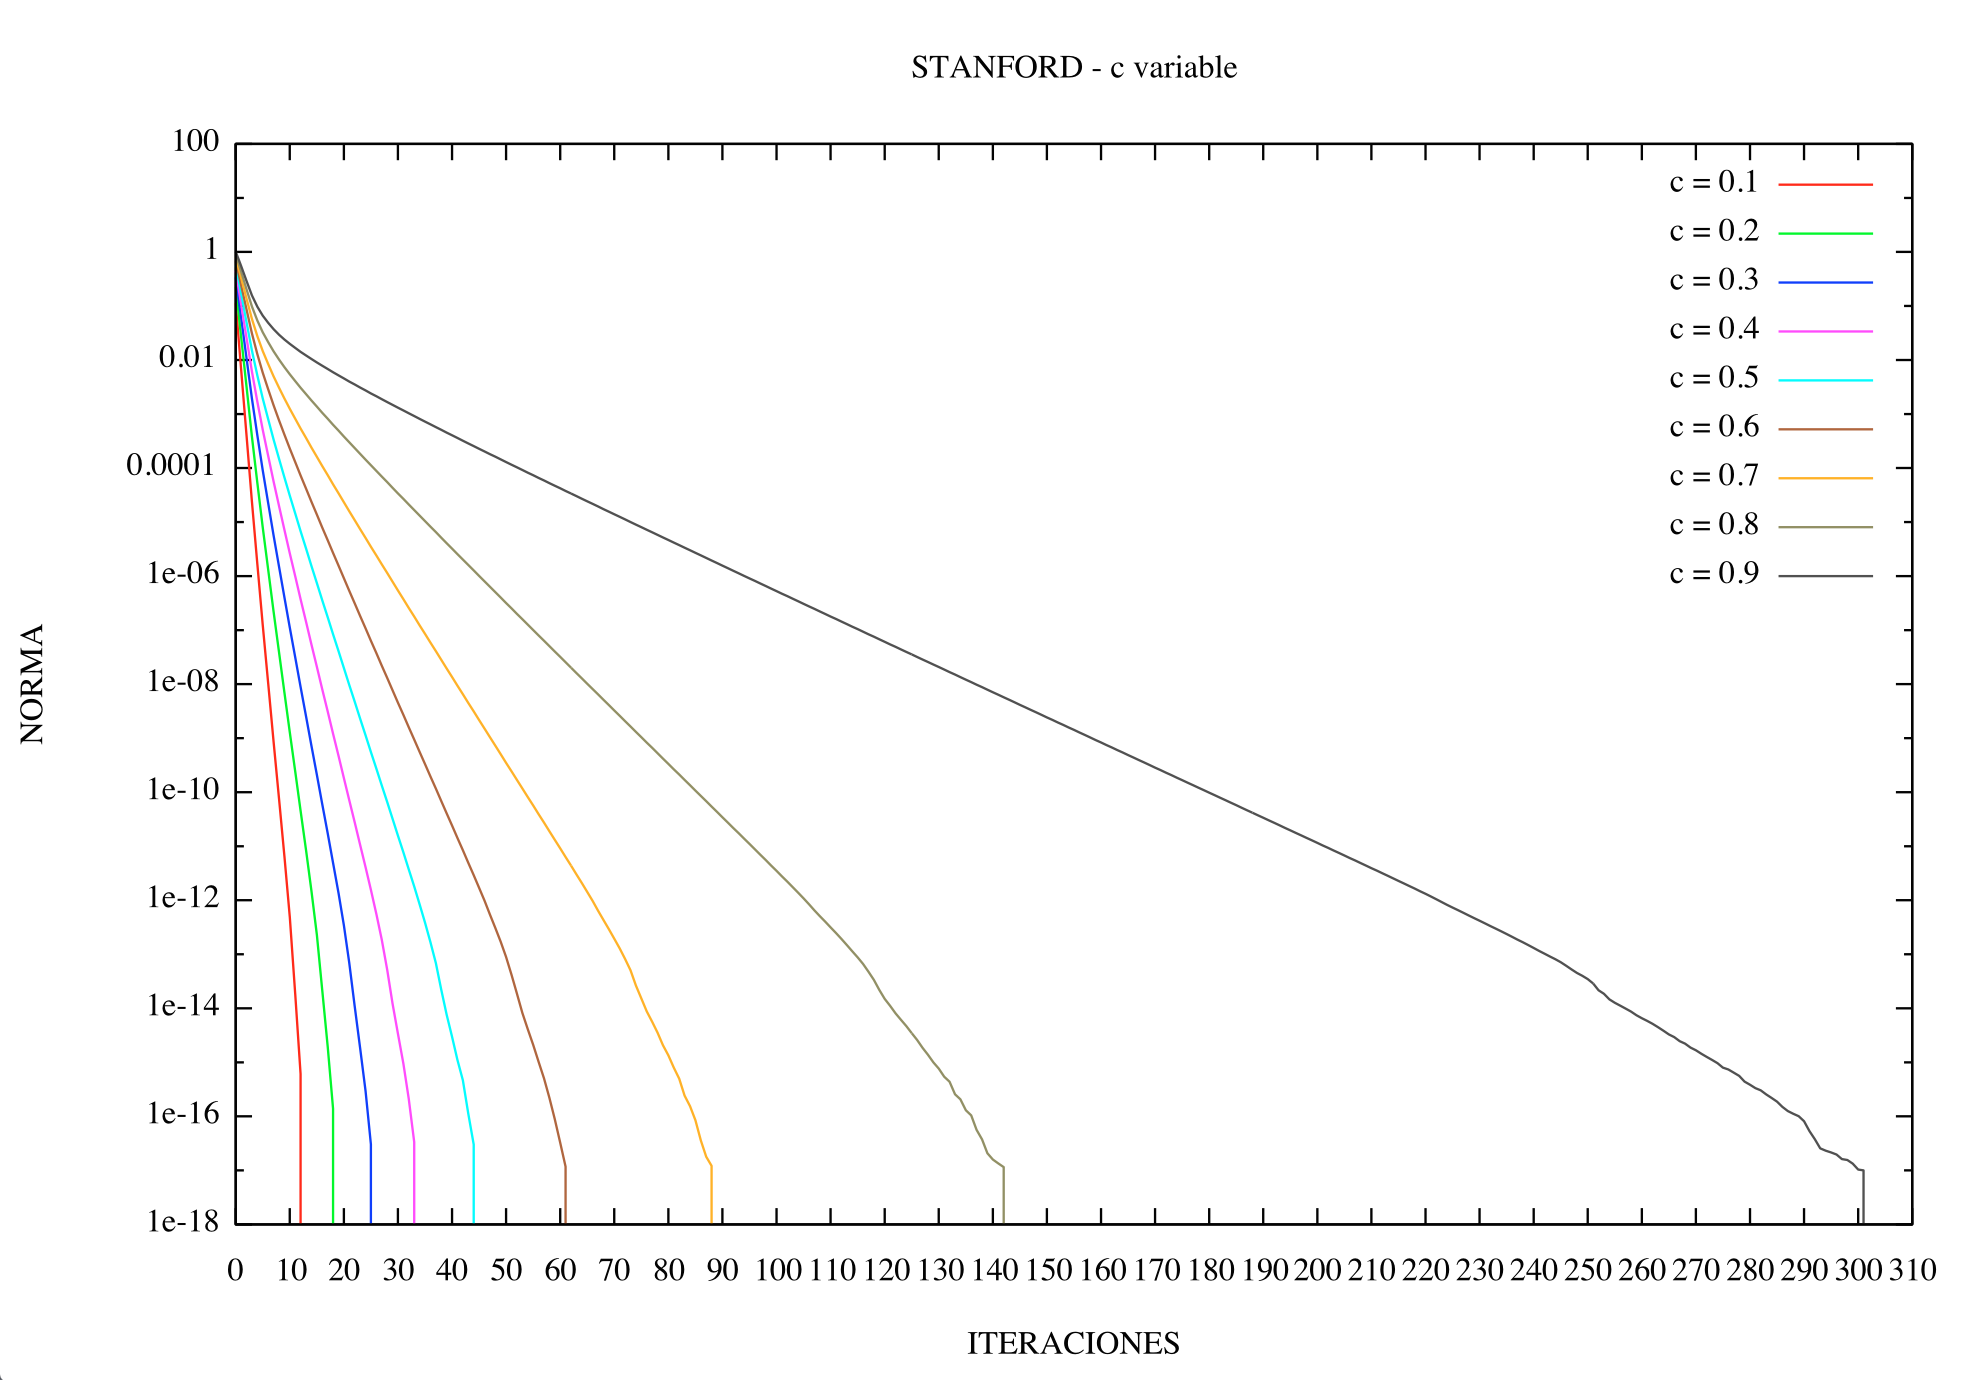
\includegraphics[scale=0.5]{imagenes/pagerank_stanford_norma.png}
    \end{center}
\end{figure}

\FloatBarrier




\subsubsection {HITS}
\subsection{Comparación de Tiempos}
 
